\section{Server (J.L.)}
\label{sec-server}

Der Server dient als Plattform für Entwicklungszwecke und zur Publikation der Weboberfläche für Externe.
Dazu wird dies auf einem \textit{Virtual Private Server}(VPS) gehostet. Der Server verfügt über das Betriebssystem Ubuntu 20.04.4 LTS \cite{ubuntu}. 
Um die Verfügbarkeit der Weboberfläche gewährleisten zu können, wird wie in Kapitel \ref{sec-Nginx} beschrieben Nginx verwendet.

\subsection{Subdomain}
Für das Projekt wurde die Subdomain \href{https://dd2.janlippemeier.de}{dd2.janlippemeier.de} mittels des folgenden Ausschnitts aus der Konfigurationsdatei von Nginx verwendt:
~\\
\begin{lstlisting}[caption={Auszug Nginx Konfiguration}, captionpos=b, label={fig:Nginx Konfiguration}]
server{
 if ($host = dd2.janlippemeier.de) {
  return 301 https://$host$request_uri;
 }
 listen 80;
 server_name dd2.janlippemeier.de;
 return 301 https://$host$request_uri;
}

server {
 server_name dd2.janlippemeier.de;
 listen              443 ssl;
 ssl_certificate /etc/letsencrypt/live/janlippemeier.de/fullchain.pem;
 ssl_certificate_key /etc/letsencrypt/live/janlippemeier.de/privkey.pem;
 location / {
  proxy_pass http://localhost:5000/;
  proxy_set_header Host             $host;
  proxy_set_header X-Real-IP        $remote_addr;
  proxy_set_header X-Forwarded-For  $proxy_add_x_forwarded_for;
  proxy_set_header X-Client-Verify  SUCCESS;
  proxy_set_header X-Client-DN      $ssl_client_s_dn;
  proxy_set_header X-SSL-Subject    $ssl_client_s_dn;
  proxy_set_header X-SSL-Issuer     $ssl_client_i_dn;
  proxy_set_header X-Forwarded-Proto https;
  proxy_read_timeout 1800;
  proxy_connect_timeout 1800;
 }
}
	
\end{lstlisting}~\\
Mit dieser Konfiguration wird mit dem ersten Server-Block bewirkt, dass sämtliche Anfragen über HTTP 
auf das sicherere Protokoll HTTPS umgeleitet werden. In dem zweiten Server Block wird dann die Funktion 
von Nginx als Reverse-Proxy genutzt. Ein Reverse-Proxy ist ein Server, der Anfragen eines Clients entgegennimmt und nach
einer internen Definition an andere Server weiterleitet. Die Antworten dieser, für den Client unbekannten, Server
werden von dem Reverse-Proxy wieder an den Client zurückgegeben. Für weitere Details wird auf die offizielle Webseite von 
Nginx zu diesem Thema verwiesen \footnote{\href{https://docs.nginx.com/nginx/admin-guide/web-server/reverse-proxy/}{Nginx Reverse Proxy Dokumentation}}
Durch diesen definierten Reverse-Proxy werden alle Anfragen an diese Subdomain intern an den Port 5000 weitergeleitet. 
Der Port 5000 muss somit nicht von außen zugänglich sein.\\
Zusätzlich wurde aus Sicherheitsgründen mit \textit{ssl\_certificate} und \textit{ssl\_certificate\_key} ein Wildcard SSL Zertifikat 
angegeben, welches eine SSL-Verschlüsselung für alle Subdomains ermöglicht.

Siehe zur Funktionsweise der verschiedenen verwendeten Nginx-Instanzen folgendes Diagramm: 

\begin{figure}[H]
    \centering
    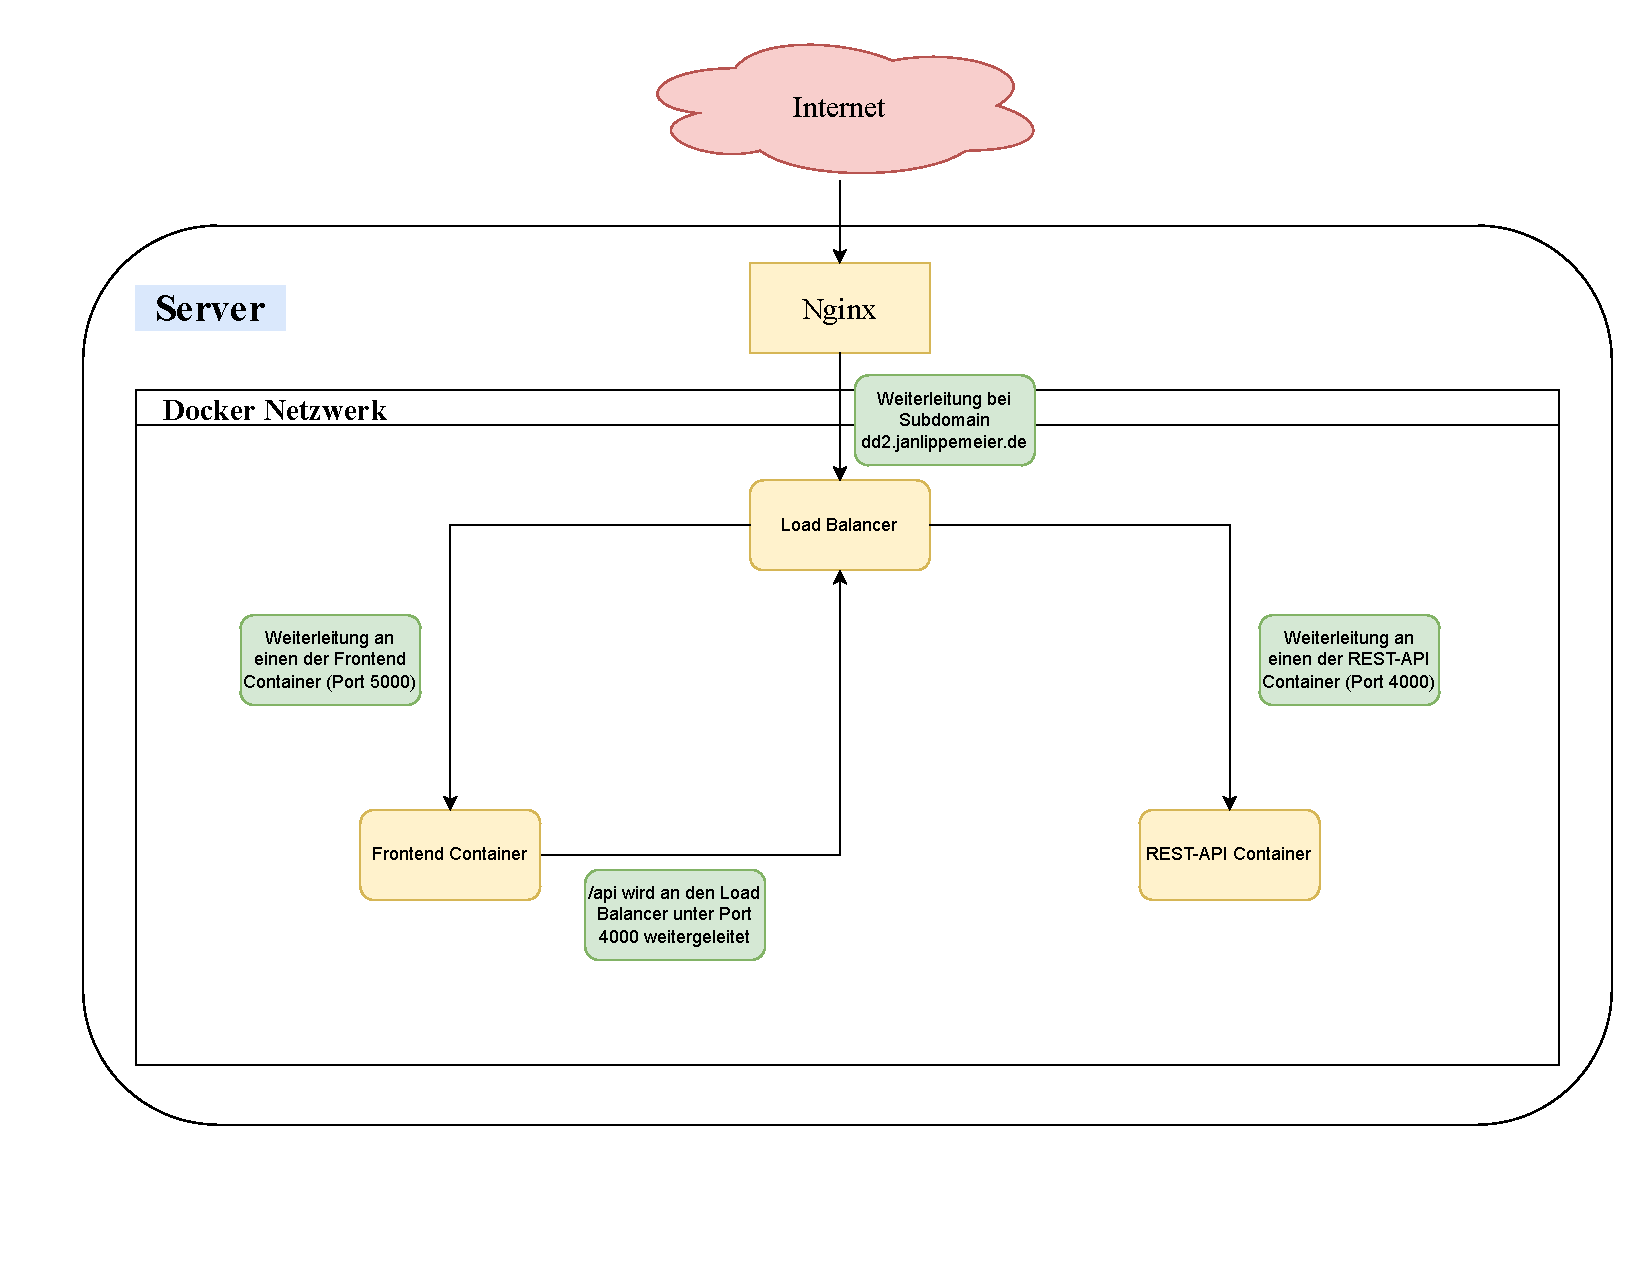
\includegraphics[width=\linewidth]{figures/NginxOverview.pdf}
    \label{fig:server}
    \caption{Nginx Konfigurationen}
\end{figure}~\\
Mit diesem Diagramm wird gezeigt, dass Requests an die Sub-Domain \href{https://dd2.janlippemeier.de}{dd2.janlippemeier.de} 
an das Docker-Netzwerk \cite{docker-network} weitergeleitet werden. Dort werden sie entsprechend vom Load-Balancer 
an den Frontend-Container weitergeleitet. Dieser gibt zum einen die HTML Seiten zur Darstellung im Browser zurück.
Zum anderen gibt der Frontend-Container Daten von Requests an die API zurück, indem die Reverse-Proxy Funktionalität 
von Nginx genutzt wird, um die Daten über den Load-Balancer von der REST-API abzufragen.

\subsection{Datensicherung}
Auf dem Server wurde mittels Cron \cite{crontab} ein, sich in regelmäßigen Intervallen wiederholender Job, nachfolgend als 
Cronjob bezeichnet, zur Datensicherung eingerichtet. Dieser Cronjob wird täglich ausgeführt und sorgt für die Erstellung 
eines Backups der Datenbank (vergleiche Kapitel \ref{sec-db}). Da es sich um ein unkritisches studentisches Projekt handelt, 
ist diese Datensicherung als Machbarkeitsbeweis anzusehen. Somit wird es nicht gemäß eines 
rationalen Best-Practices auf einem anderen System gespeichert. 

\subsubsection{Backup Erstellung}
Zur Installation von postgres \cite{postgresql} und somit des Befehls \textit{pg\_dump} auf dem VPS wird der 
folgende Befehl verwendet:
~\\\begin{lstlisting}[caption={Befehl zum Installieren von PostgreSQL}, captionpos=b, label={fig:PostgreSQL Installation}]
sudo apt install postgresql
\end{lstlisting}
~\\ \textit{pg\_dump} ist ein Kommando-Zeilen-basierter Befehl zum Erstellen von Backups. 
Um das Passwort zu hinterlegen wird eine Umgebungsvariable mit dem Namen \textit{PGPASSWORD} 
erstellt, die das Passwort für den Admin Nutzer enthält. Die Erstellung eines Backups erfolgt über den Befehl: 
~\\\begin{lstlisting}[caption={Backup Befehl}, captionpos=b, label={fig:Backup Command}]
pg_dump 
    -h localhost 
    -U postgres 
    DB_WATER 
    | gzip 
    > "/Backup/DD2/backup`date +\%Y-\%m-\%dT\%H:\%M:\%S`.gz"
\end{lstlisting}
~\\Durch den folgenden Befehl wird der von \textit{pg\_dump} zurückgelieferte String unter 
Verwendung von \textit{gzip} komprimiert. 
~\\\begin{lstlisting}[caption={Komprimieren des Backups}, captionpos=b, label={fig:gzip pipe}]
    | gzip > 
\end{lstlisting}
~\\ Dieser komprimierte String wird in eine Datei mit dem im Befehl nachfolgend spezifizierten 
Dateinamen geschrieben. \\
Der mit \textit{"/Backup/DD2/backup`date +\%Y-\%m-\%dT\%H:\%M:\%S`.gz"} spezifizierte Dateiname 
besteht aus dem Wort \textit{backup} gefolgt von dem aktuellen Zeitstempel und der Dateiendung 
\textit{.gz}, die anzeigt, dass die Datei mittels gzip komprimiert wurde. Diese Datei wird in 
dem Ordner mit dem Pfad \textit{/Backup/DD2} gespeichert.

\subsubsection{Einrichtung von Cron}
Cron wurde auf dem VPS mittels des folgenden Befehls installiert: 
~\\\begin{lstlisting}[caption={Befehl zum Installieren von cron}, captionpos=b, 
    label={fig:Cron Installation}]
    sudo apt install cron
\end{lstlisting}
~\\ Cron ist ein Tool zum Anlegen der genannten Cronjobs. Damit regelmäßig die 
Cronjobs ausgeführt werden können, wird mittels des Befehls \textit{sudo systemctl enable cron} 
die Ausführung im Hintergrund erlaubt. Durch den folgenden Befehl wird ein neuer Cronjob angelegt: 
~\\\begin{lstlisting}[caption={Befehl zum Erstellen eines neuen Cronjobs}, captionpos=b, 
    label={fig:CronJob Creation}]
    crontab -e
\end{lstlisting}
~\\ Um die Häufigkeit der Ausführungen zu definieren wird die folgende Definition verwendet, die 
dafür sorgt, dass der danach eingegebene Befehl zum Erstellen eines Backups täglich um 04:00
morgens ausgeführt wird: 
~\\\begin{lstlisting}[caption={Definition des Ausführungsintervalls}, captionpos=b, 
    label={fig:CronJob Definition}]
    0 4 * * *
\end{lstlisting}